\documentclass[../dissertation.tex]{subfiles}
 
\begin{document}

\section{Experiment 2}

	This experiment tested the core hypothesis of this dissertation. I used a within-subjects design to test whether executive function is specifically related to categorization in the hypothesis-testing system while verbal labels are specifically related to associative system categorization. This experiment also uses three different category learning tasks, which allowed me to compare different category learning paradigms and to test the core hypothesis for multiple approaches. \par
	In this experiment, I use vocabulary as a proxy for labeling. Vocabulary measures should reflect the link between a word and its meaning, as individuals must retrieve the meaning of a word from its label in the task. Further, this link should be more elaborated than those built in a paired-associate learning task. Thus, individual differences in vocabulary should give some insight into how well participants use labels in learning categories. For executive function, I selected three different measures. Multiple studies have shown that while executive function is sometimes talked about as a single construct, it actually is made up of separable components \citep{Miyake2000, Karr2018}. The components I chose to focus on were inhibition, switching, and planning. I made this decision in an effort to have some breadth in executive function measurements. \par
	Finally, I chose to compare the COVIS, statistical density, and taxonomic/thematic approaches to category learning. These three approaches represent a broad spectrum of category learning. COVIS exclusively focuses on perceptual categories, while the statistical density approach uses constructed stimuli that can be mapped onto real-world objects to some degree. Finally, the taxonomic/thematic approach is almost always applied to real-world objects that participants have directly experienced. Since these three approaches are so different in the types of categories they try to explain, results showing similarities between them would be strong evidence for an overarching dual-systems framework. I decided to use common paradigms from each approach as a starting point for comparison rather than modifying the tasks to be more equivalent. Given the theoretical similarities between the approaches, I hypothesize that task differences will not be sufficient to affect how individuals use the two systems differently for each approach.

\subsection{Method}
\subsubsection{Participants}
186 participants were recruited from the psychology undergraduate participant pool at the University of Connecticut (135 Female, 50 Male, mean age = 18.72). Not all subjects were used for all analyses; see descriptions of each analysis for more details.
\subsubsection{Category learning tasks}
This experiment used three different category learning tasks, each based on a different approach to category learning. I used these three tasks to investigate whether the paradigms used in different approaches engage category learning systems in a similar way. The order of category learning tasks was counterbalanced across participants. All category learning tasks were presented using PsychoPy v.1.84.2 \citep{Peirce2007}. \par 
\textbf{Sloustky statistical density task.} This task used the same procedure and stimuli as the task described in Experiment 1. However, instead of completing only two blocks, participants completed all four blocks. Because the previous experiment showed few significant order effects, the order of the four blocks was randomly generated for each participant. \par
\textbf{Ashby perceptual category learning task.} There were two versions to this task: Information-Integration (II) and Rule-Based (RB). Participants completed the II version and then the RB version. Prior research has shown that when participants are asked to switch between the declarative (hypothesis-testing) and implicit (associative) systems, they end up using rule-based strategies from the declarative system for all trials. Thus, by engaging the implicit system first, I aimed to reduce transfer effects between versions as much as possible. \par

\begin{wrapfigure}{L}{0.625\textwidth}
\vspace{-10pt}
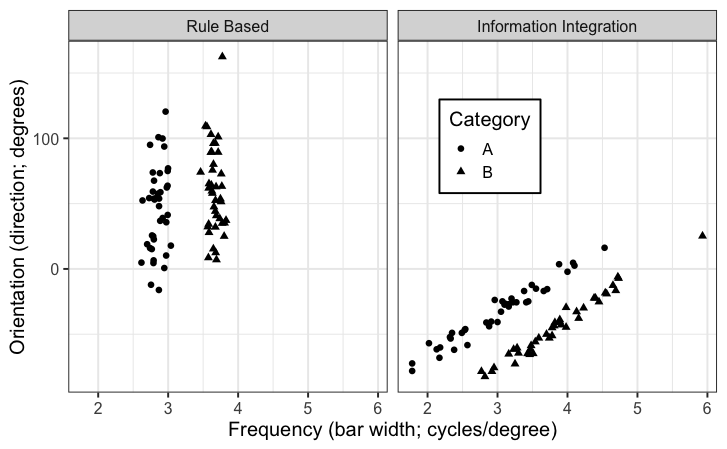
\includegraphics[scale=0.40]{ashby_stim.png}
\caption[Stimulus parameters for Ashby perceptual category learning task]{Parameters for Gabor patches for each version of the Ashby perceptual category learning task. }
\label{ashby_param}
\vspace{-20pt}
\end{wrapfigure}	


In each version of the task, participants were told that they would be learning two categories and that perfect performance was possible. They were also told to be as quick and accurate as possible. In each trial, participants viewed a Gabor patch that belonged to one of the two categories. Each patch subtended 11\degree  of visual angle. The stimuli were generated using category parameters from a prior study (\citealp{Maddox2003}; see Figure \ref{ashby_param} for details).  The participant then had 5000ms to press a key, indicating which category they believed the stimulus belonged to. After a response, the participant received feedback ("Correct" or "Incorrect"). Feedback was presented for 1000ms, and then the next trial began. If the participant took more than 5000ms to respond, they saw "Too Slow" and proceeded to the next trial. Participants completed three runs of each version. Each run had 80 trials (40 from each category) presented in a random order. Thus, in total participants completed 240 II trials and 240 RB trials. \par
\textbf{Taxonomic/thematic task.} This task was adapted from \citet{Murphy2001} and \citet{Kalenine2009}. There were also two versions of this task: one taxonomic and one thematic. Version order was counterbalanced across subjects, with some participants getting the taxonomic version first and others the thematic version first. Most versions of this type of task allow participants to choose the item that is most "semantically related," and thus do not ask participants to make either taxonomic or thematic choices on any given trial. As such, little research has looked at switching between taxonomic and thematic semantic judgments. Counterbalancing was applied to control for order effects. \par
The stimuli were images taken from \citet{Konkle2010}. I chose to use images in order to avoid automatic language processing. While participants likely did engage linguistic resources during the task, the use of pictures reduced the influence of stimulus features on language use. In each trial, four images were presented: a target, a taxonomically-related item, a thematically-related item, and an unrelated item. Taxonomically- and thematically-related items were chosen based on norms from \citet{Landrigan2016} where available. The \citet{Landrigan2016} norms were based on word stimuli rather than the images available from \citet{Konkle2010}; as such, not all of the available images were normed. For images without norming information, researcher judgment was used to pick items for each type of relation. \par
For each version, participants were told that they would be categorizing objects. They were told to pick the option that "goes best with" (thematic) or is "most similar to" (taxonomic) the target item. These instructions were based on previous research showing that slight differences in task instructions affect taxonomic and thematic judgments \citep{Lin2001}. After instructions, participants got five practice trials. In each trial, the images were shown for 5000ms and participants had unlimited time to make a response. The practice trials were identical for the taxonomic and thematic versions of the task. After each response, participants received feedback ("Correct!" or "Oops!") for 1000ms. Once the practice trials were completed, participants received 24 test trials. Test trials had the same feedback structure as practice trials. While some images were seen in multiple trials, the 4-image combination for each trial was unique across the taxonomic and thematic versions of the task.
\subsubsection{Executive function tasks} 
To measure executive function, I used three different tasks taken from the Psychology Experiment Building Language (PEBL) test battery \citep{Mueller2014}. I chose three tasks to try and tap multiple aspects of executive function, including inhibition, planning, and task-switching. All three tasks were presented using the PEBL software.\par
\textbf{Flanker task (inhibition).} This task was an implementation of the \citet{Eriksen1979} flanker task, using a method similar to \citet{Stins2007}. In each trial, participants viewed a set of five arrows and were asked to respond based on the direction in which the center arrow was pointing (left or right). In congruent trials, all arrows faced the same way. In incongruent trials, the four distractor arrows pointed in the opposite direction of the target (center) arrow. In neutral trials, the four distractor arrows were just horizontal lines without arrowheads. There were also blank trials, in which only the target arrow appeared. Participants completed 40 trials in a 2 (direction; left, right) x 4 (condition; congruent, incongruent, neutral, blank) design, for a total of 160 trials. Each trial began with a 500 ms fixation, followed by the stimulus which appeared for 800ms. Participants were only allowed to respond during the 800ms that the stimulus was on the screen. After a response, there was an inter-trial interval of 1000ms. Participants received 8 practice trials before the actual experiment to get used to the timing constraints. During practice trials, each response was followed by feedback ("Correct", "Incorrect") as well as a number indicating RT for that trial. This feedback was not provided for the test trials. \par
\textbf{Switcher task (task-switching).} This task was taken from \citet{Anderson2012}. In this task, participants were presented with an array of colored shapes. Each colored shape had a single letter inside. For each trial, a single shape was surrounded by a white circle, indicating it as the target shape. Based on instructions at the top of the screen, participants were told to select a new shape that matched the target shape on one of three dimensions (color, shape, or letter). Research from \citet{Miyake2004} has shown that cueing a dimension using its entire name (e.g. "shape") does not require as many language resources as cueing a dimension using a single letter (e.g., "s"). Since one of the core hypotheses of this study was that language supports executive functions in the hypothesis-testing system, I used a version of the switcher task that cued dimension using just a single letter. I expect that this version of the task requires individuals to represent dimensions/selection rules internally, similar to how they might represent possible category rules when learning rule-based categories. \par
The task consisted of nine different arrays of ten shapes. For each array, participants made ten responses. In the first three arrays, participants switched between two of the three dimensions in a fixed order (e.g., C - S - C - S). The relevant dimensions were different for each array. For the second three arrays, participants switched between all three dimensions still in a fixed order (e.g., S - C - L - S - C - L). The specific order was different for each array. Finally, in the last three arrays participants switched between all three dimensions in a random order. Unlike previous arrays, in the last three participants were unable to anticipate the upcoming relevant dimension. Each array had 12 cues. \par
\textbf{Tower of London task (planning)}. This task was a computerized version of the one described in \citet{Shallice1982}. In this task, participants were shown a setup of colored disks in three stacks as well as a target setup. They were given a limited number of moves to make their setup match the target setup. Participants could only have one disk in their "hand" at a time, and they could only pick the top disk up off of any stack. The trials varied in the number of steps required to match the target setup from 2 to 5, with easier (2 step) trials at the beginning of the task and harder (5 step) trials at the end of the task. Participants were encouraged to take their time and plan out their moves before beginning each trial. There were a total of 12 trials.

\subsubsection{Behavioral measures} 
Finally, I used four different behavioral assessments to measure vocabulary, syntax, and nonverbal IQ.
\textbf{Nelson-Denny vocabulary subtest.} To measure vocabulary, I used the same Nelson-Denny vocabulary subtest described in Experiment 1. \par
\textbf{Clinical Evaluation of Language Fundamentals recalling sentences and formulated sentences subtests}. I used the CELF here to measure individual differences in syntax production and perception. The Recalling Sentences subtest provided a measure of receptive grammar, while the Formulated Sentences subtest measured expressive grammar. See Experiment 1 for a description of the Recalling Sentences subtest. In the Formulated Sentences subtest, participants viewed a scene and were asked to make a sentence containing a target word about that scene. Often, the target word encouraged certain syntactic structures (e.g., "because"). Raw scores were calculated based on use of the target word and errors in syntax or semantics for each item. Like Recalling Sentences, Formulated Sentences were converted to standard scores with a mean of 10 and a standard deviation of 3. \par
\textbf{Raven's Advanced Matrices.} I used Raven's Advanced matrices to measure nonverbal IQ, as described in Experiment 1.

\subsubsection{Procedure}

Each participant completed all of the category learning and executive function tasks, as well as all of the behavioral measures. CELF responses were audio-recorded to allow for offline scoring. To allow multiple subjects to be run in a single timeslot, some participants received tasks in a shuffled order. All together, the tasks and behavioral measures took about an hour and a half.

\subsection{Results I: individual differences}

Descriptive statistics for all individual difference measures can be found in Table \ref{iddesc}.

\begin{table}[H]
\caption{Descriptive statistics for individual difference measures.}
\vspace{-10pt}
\begin{center}
\begin{tabularx}{\textwidth}{>{\centering\arraybackslash}p{7cm}>{\centering\arraybackslash}p{1.5cm}YYY}
\toprule
Measure                   & Mean & SD    & Range        \\
\midrule
Flanker Effect            & 55.2 & 27.3  & -37.5-155    \\
Switcher Effect           & 8026 & 13729 & -28119-51916 \\
Tower of London Accuracy  & 0.66 & 0.18  & 0.083-1.00   \\
Nelson-Denny Vocab        & 230  & 14.2  & 177-255      \\
Raven's Advanced Matrices & 15.1 & 4.73  & 0-26         \\
CELF Recalling Sentences  & 11.1 & 1.68  & 6-14         \\
CELF Formulated Sentences & 12.5 & 1.17  & 9-14        \\
\bottomrule
\end{tabularx}
\label{iddesc}
\end{center}
\vspace{-10pt}
\small\textit{Note}. This table includes data from all 186 participants. Flanker and switcher effect measures are reported in milliseconds. Nelson-Denny Vocab and both CELF measures are standard scores.
\end{table}

Descriptive statistics for the category learning tasks can be found in Tables \ref{exp2_catlearn_acc_desc} and \ref{exp2_catlearn_rt_desc}. These statistics describe accuracy and reaction time aggregated by subject and block. For a review on which block corresponds to which system in each paradigm, see Table \ref{exp2systems}.

\begin{table}[H]
\caption{Descriptive statistics for category learning tasks -- accuracy.}
\vspace{-10pt}
\begin{center}
\begin{tabularx}{\textwidth}{>{\centering\arraybackslash}p{4.5cm}YYYYYY}
\toprule
\multirow{2}{*}{Paradigm}    & \multicolumn{3}{c}{Associative} & \multicolumn{3}{c}{Hypothesis-testing} \\
                             & Mean    & SD      & Range       & Mean      & SD        & Range          \\
\midrule
Ashby perceptual             & 0.58    & 0.07    & 0.44-0.78 & 0.78      & 0.16      & 0.42-0.98     \\
Sloutsky statistical density & 0.95    & 0.08    & 0.60-1.00 & 0.93      & 0.12      & 0.20-1.00     \\
Taxonomic/thematic           & 0.83    & 0.16    & 0.13-1.00 & 0.85      & 0.15      & 0.21-1.00     \\
\bottomrule 
\label{exp2_catlearn_acc_desc}
\end{tabularx}
\end{center}
\vspace{-10pt}
\small\textit{Note}. This table includes data from all 186 participants.
\end{table}

\begin{table}[H]
\caption{Descriptive statistics for category learning tasks -- reaction time.}
\vspace{-10pt}
\begin{center}
\begin{tabularx}{\textwidth}{>{\centering\arraybackslash}p{4.5cm}YYYYYY}
\toprule
\multirow{2}{*}{Paradigm}    & \multicolumn{3}{c}{Associative} & \multicolumn{3}{c}{Hypothesis-testing} \\
                             & Mean    & SD      & Range       & Mean      & SD        & Range          \\
\midrule
Ashby perceptual             & 739    & 0241    & 154-1780 & 625      & 141      & 152-1040   \\
Sloutsky statistical density & 766    & 196     & 413-1380 & 658      & 144      & 380-1210 \\
Taxonomic/thematic           & 1620    & 649    & 264-6030 & 1780      & 557      & 558-4280     \\
\bottomrule 
\label{exp2_catlearn_rt_desc}
\end{tabularx}
\end{center}
\vspace{-10pt}
\small\textit{Note}. This table includes data from all 186 participants. Reaction times are reported in milliseconds.
\end{table}

\subsubsection{Data processing}
	An \textit{a priori} power analysis showed that 132 subjects would be needed for the individual difference analyses. As is noted above, more than 132 subjects participated in the experiment. Due to the many assessments being collected, issues with the experimental paradigm, and experimental time constraints, there was a considerable amount of data missingness. Thus, each analysis discussed below uses the first 132 subjects with full data for all measures included in that analysis. \par
	\textbf{Ashby perceptual category learning task.} For this task, II blocks were labeled as associative and RB as hypothesis-testing. Accuracy and reaction time were measured for this task. Accuracy was summarized by subject and system. For reaction time, only accurate trials were used. In addition, reaction times that were recorded as a negative value were removed, as these trials indicate a participant pressed a key before the stimulus appeared. Then, outliers were removed on a by-trial basis by calculating the mean and standard deviation of reaction times within a given subject and system. Any trial with a reaction time more than 2 SDs away from the mean was discarded. Then, reaction time was summarized by subject and system. A single subject had reaction times 8 SD higher than the mean; this subject's data was removed and replaced with another subject. Accuracy and reaction time were then Yeo-Johnson transformed to reduce skewness, as well as centered and scaled. \par
	\textbf{Sloutsky statistical density task.} In this task, the unsupervised-dense block was considered to engage the associative system, and the supervised-sparse block was considered to engage the hypothesis-testing system. The other two blocks were discarded. Any participants who did not respond correctly to at least 6 of the 8 catch trials for a given block were removed from future analyses. Thus, all subjects reported in analyses using this task had at least 75\% accuracy on catch trials in both blocks. Accuracy was summarized by subject and system. Reaction time outliers were removed on a by-trial basis as described above and reaction time was then summarized by subject and system. Accuracy and reaction time were then transformed, centered, and scaled. \par
	\textbf{Taxonomic/thematic task.} For this task, taxonomic blocks were associative and thematic blocks were hypothesis-testing. Practice trials were discarded before analysis. Accuracy was summarized by subject and system. Reaction time outliers were removed using the same method as above, and then reaction time was summarized by subject and system. Accuracy and reaction time were then transformed, centered, and scaled. \par

\begin{table}[H]
\caption{Associative and hypothesis-testing blocks for each paradigm.}
\vspace{-10pt}
\begin{center}
\begin{tabularx}{\textwidth}{>{\centering\arraybackslash}p{5cm}YY}
 \toprule
Paradigm                     & Associative             & Hypothesis-testing \\
\midrule
Ashby perceptual             & Information-integration & Rule-based         \\
Sloutsky statistical density & Unsupervised-Dense      & Supervised-Sparse  \\
Taxonomic/thematic           & Taxonomic               & Thematic  \\
 \bottomrule 
\end{tabularx}
\label{exp2systems}
\end{center}
\end{table}
	
	\textbf{Flanker task.} The flanker effect was calculated by first selecting only incongruent or congruent trials. Then, the average reaction time for each trial type was calculated by subject. Finally, the average reaction time for congruent trials was subtracted from the average reaction time for incongruent trials for each subject. This measure reflecting the flanker effect was then centered and scaled but not transformed, as it was not shown to be significantly skewed. \par
	\textbf{Switcher task.} The switcher effect was calculated by selecting the arrays in the 3-dimension ordered and 3-dimension random blocks. Within each array, the median reaction time for each cue was calculated. Then, average reaction time was calculated for each block. Finally, the reaction time for 3-dimension ordered was subtracted from the reaction time for 3-dimension random. This measure was then transformed, centered, and scaled. \par 
	\textbf{Tower of London task.} The metric calculated for this task was percentage of trials correct. This measure was then transformed, centered, and scaled. \par 
	\textbf{Nelson-Denny, CELF, RAM}. Nelson-Denny and CELF were both standardized using their respective norms. Raven's was not standardized. All 4 measures (Nelson-Denny vocabulary, CELF Recalling Sentences, CELF Formulated Sentences, and Raven's Advanced Matrices) were all transformed, centered, and scaled.
	
\begin{table}[H]
\caption{Correlations between individual difference measures.}
\vspace{-10pt}
\begin{center}
\begin{tabularx}{\textwidth}{p{6cm}YYYY}
\toprule
\multicolumn{1}{c}{Measure}  & 1     & 2     & 3     & 4     \\
\midrule
1. Nelson-Denny Vocab        & -     &       &       &       \\
2. Tower of London Accuracy  & 0.21  & -     &       &       \\
3. Switcher Effect           & -0.06 & -0.03 & -     &       \\
4. Flanker Effect            & -0.05 & -0.06 & 0.08  & -     \\
5. Raven's Advanced Matrices & 0.44* & 0.26* & -0.19 & -0.04\\
\bottomrule
\end{tabularx}
\label{exp2id_corr}
\end{center}
\vspace{-10pt}
\small\textit{Note}. *\textit{p}\textless 0.05, Bonferroni-corrected. This table includes data from all 186 participants.
\end{table}
	
\newpage
\subsubsection{Accuracy}

\begin{wrapfigure}{R}{0.625\textwidth}
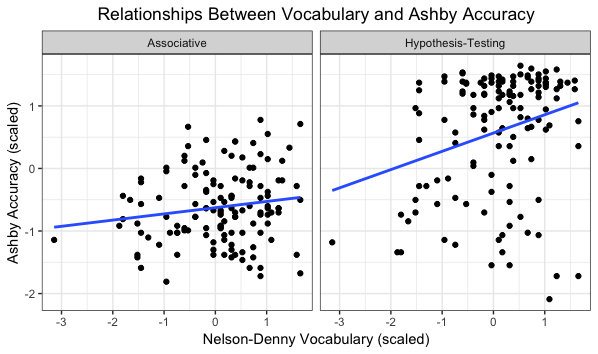
\includegraphics[scale=0.5]{ashby_acc_vocab.png}
\caption[Relationships between Ashby accuracy and vocabulary]{Vocabulary is a significant predictor of accuracy in the Ashby perceptual category learning task for the hypothesis-testing block, but not for the associative block.}
\label{ashby_acc_vocab}
\vspace{-30pt}
\end{wrapfigure}	

\textbf{Ashby perceptual category learning task.} To investigate how the individual difference measures related to task performance, I constructed a mixed-effects model with random intercepts for subject. Adding the fixed effect of system significantly improved model fit,  $\chi^{2}(1)$ = 138.15, p \textless 0.0001. In the next step, I added RAM, vocabulary, and the three executive function tasks as fixed effects. This further improved fit, $\chi^{2}(5)$ = 12.24, p = 0.03. Next, I added the interactions between the individual difference measures (vocabulary, flanker, switcher, and Tower of London) and system one by one. The only interaction that significantly improved fit was the between vocabulary and system, $\chi^{2}(1)$ = 4.82, p = 0.03. Thus, the final model included random intercepts for subject, fixed main effects for system, RAM, vocabulary and all three executive function tasks, and the fixed interaction effect between vocabulary and system. This model revealed a significant interaction between vocabulary and system, \textit{F}(1,131) = 4.83, \textit{p} = 0.03 (see Fig \ref{ashby_acc_vocab}). The model also revealed significant main effects of system and vocabulary. \par 
	To break down the interaction, I ran separate follow-up linear models for each of the systems. Vocabulary remained a significant predictor in the hypothesis-testing model, \textit{F}(1,126) = 7.36, \textit{p} = 0.004. The coefficient associated with vocabulary in this model was positive (\textit{b} = 0.29, \textit{SE} = 0.10). However, vocabulary was not a significant predictor in the associative model, \textit{F}(1,127) = 1.16, \textit{p} = 0.28. Thus, participants with higher vocabularies showed higher accuracy in the hypothesis-testing block, but accuracy was not related to vocabulary in the associative block. \par	
	\textbf{Sloutsky statistical density task.}  To investigate how the individual difference measures related to task performance, I constructed a mixed-effects model with random intercepts for subject. Adding the fixed effect of system marginally improved model fit,  $\chi^{2}(1)$ = 3.38, p = 0.07. In the next step, I added RAM, vocabulary, and the three executive function tasks as fixed effects. This step significantly improved fit, $\chi^{2}(5)$  = 17.27, \textit{p} = 0.004. In the next steps, I added each of the interactions between individual difference measures and system one by one. None of the interactions improved fit. Thus, the final model predicted accuracy in this task from system and the individual difference measures, but not their interactions. This model revealed a significant main effect of flanker, \textit{F}(1,126) = 4.34, \textit{p} = 0.04, and a significant main effect of switcher, \textit{F}(1,126) = 8.87, \textit{p} = 0.003 (see Fig \ref{sl_acc_eff}). 	

\begin{wrapfigure}{L}{0.45\textwidth}
\vspace{-10pt}
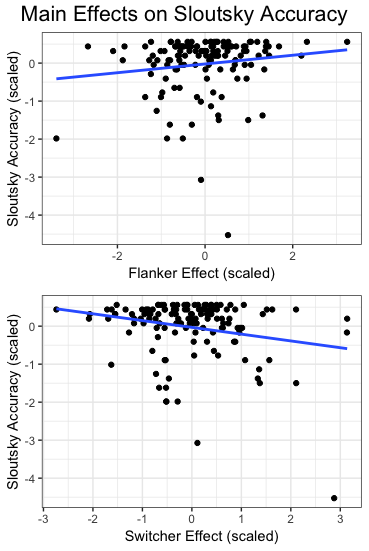
\includegraphics[scale=0.55]{sl_acc_eff.png}
\caption[Main effects of flanker and switcher on Sloutsky accuracy]{Flanker performance has a positive relationship with Sloutsky accuracy, while switcher performance has a negative one. Sloutsky accuracy is collapsed across blocks.}
\label{sl_acc_eff}
\vspace{-20pt}
\end{wrapfigure}		
	
	The coefficient associated with flanker was positive (\textit{b} = 0.14, \textit{SE} = 0.07), while the coefficient associated with switcher was negative, (\textit{b} = -0.20, \textit{SE} = 0.07). There was also a marginally significant effect of system, \textit{F}(1,131) = 3.40, \textit{p} = 0.07. Thus, accuracy on the Sloutsky statistical density task was positively related to flanker performance and negatively related to switcher performance. However, these results should be interpreted with caution, as large ceiling effects were found in accuracy for this task. \par
	
\begin{wrapfigure}{R}{0.5\textwidth}
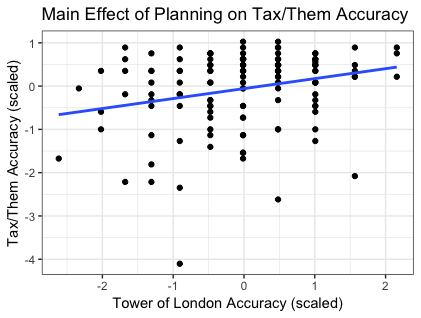
\includegraphics[scale=0.55]{tt_acc_tol.png}
\caption[Main effect of planning on taxonomic/thematic accuracy]{Tower of London accuracy is positively related to accuracy in the taxonomic/thematic task. Taxonomic/thematic accuracy is collapsed across blocks.}
\label{tt_acc_tol}
\vspace{-10pt}
\end{wrapfigure}	

	\textbf{Taxonomic/thematic task.}  Again I constructed a mixed-effects model with random intercepts for subject. Adding the fixed effect of system significantly improved model fit,  $\chi^{2}(1)$ = 5.13, p = 0.002. Adding the individual difference measures also significantly improved fit, $\chi^{2}(5)$  = 12.31, \textit{p} = 0.03. None of the interactions significantly improved fit. Thus, the final model predicted accuracy in this task from system and the individual difference measures, but not their interactions. This model revealed a significant main effect of system, \textit{F}(1,131) = 5.20, \textit{p} = 0.02, and a significant main effect of Tower of London, \textit{F}(1,126) = 6.56, \textit{p} = 0.01 (see Fig \ref{tt_acc_tol}). The coefficient associated with Tower of London was positive (\textit{b} = 0.20, \textit{SE} = 0.08). Thus, accuracy on the taxonomic/thematic task was positively related to performance on Tower of London. \par
	\textbf{Summary.} This section showed that different individual difference measures were related to accuracy in the three category learning tasks. In the Ashby perceptual category learning task, there was a specific positive effect of vocabulary on performance in the hypothesis-testing block. For the Sloutsky statistical density task, accuracy was positively related to flanker performance and negatively related to switcher performance. Tower of London accuracy was positively related to accuracy in the taxonomic/thematic task.

\subsubsection{Reaction time}

\textbf{Ashby perceptual category learning task.}  To investigate how the individual difference measures were related to reaction time, I constructed a mixed-effects model with random intercepts for subject. Adding the fixed effect of system significantly improved model fit,  $\chi^{2}(1)$ = 33.97, p \textless 0.0001. In the next step, I added fixed effects of all of the individual difference measures and RAM. This further improved fit, $\chi^{2}(5)$ = 12.18, p = 0.03. Next, I added the interactions one by one. The only interaction that significantly improved fit was the between vocabulary and system, $\chi^{2}(1)$ = 11.19, p = 0.0008. Thus, the final model included random intercepts for subject, fixed main effects for system, RAM, vocabulary and all three executive function tasks, and the fixed interaction effect between vocabulary and system. This model revealed a significant interaction between vocabulary and system, \textit{F}(1,130) = 11.49, \textit{p} = 0.0009 (see Fig \ref{ashby_rt_vocab}). The model also revealed significant main effects of system and vocabulary and a marginal main effect of Tower of London. \par 


\begin{wrapfigure}{R}{0.675\textwidth}
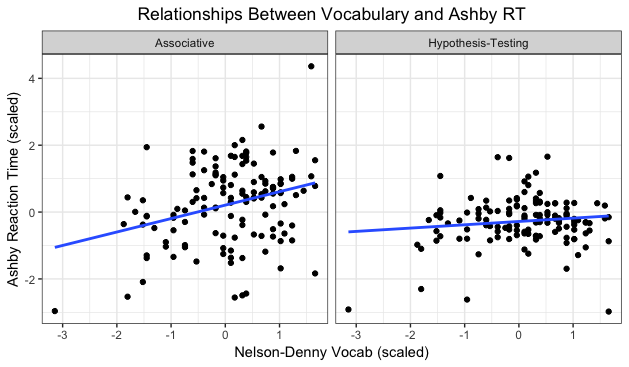
\includegraphics[scale=0.5]{ashby_rt_vocab.png}
\caption[Relationships between Ashby reaction time and vocabulary]{Vocabulary is a significant predictor of reaction time in the Ashby perceptual category learning task for the associative block, but not for the hypothesis-testing block.}
\label{ashby_rt_vocab}
\vspace{-10pt}
\end{wrapfigure}	


	To break down the interaction, I ran separate follow-up linear models for each of the systems. For reaction time, vocabulary was not a significant predictor in the hypothesis-testing model, \textit{F}(1,125) = 1.49, \textit{p} = 0.23.  However, vocabulary was a significant predictor in the associative model, \textit{F}(1,125) = 10.41, \textit{p} = 0.002. The coefficient associated with vocabulary in this model was positive (\textit{b} = 0.40, \textit{SE} = 0.12). Thus, participants with higher vocabularies showed slower reaction times in the associative block, but reaction time was not related to vocabulary in the hypothesis-testing block.\par 
	
\begin{wrapfigure}{L}{0.6\textwidth}
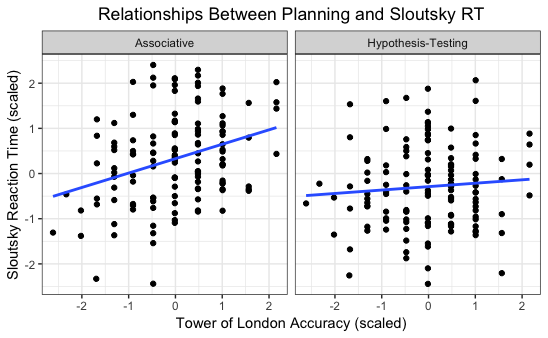
\includegraphics[scale=0.5]{sl_rt_tol.png}
\caption[Relationships between Sloutsky reaction time and planning]{Tower of London accuracy is a significant predictor of reaction time in the Sloutsky statistical density task for the associative block, but not for the hypothesis-testing block.}
\label{sl_rt_tol}
\vspace{-10pt}
\end{wrapfigure}	

\textbf{Sloutsky statistical density task.}  Once again I constructed a mixed-effects model with random intercepts for subject. Adding the fixed effect of system significantly improved model fit,  $\chi^{2}(1)$ = 52.75, p \textless 0.001. Adding the individual difference measures as fixed effects also significantly improved fit, $\chi^{2}(5)$ = 12.35, \textit{p} = 0.03. The only interaction that significantly improved fit was between system and Tower of London, $\chi^{2}(1)$ = 10.17, p = 0.001. Thus, the final model had the fixed effects of system and the individual difference measures as well as the interaction between system and Tower of London. This model showed a significant interaction between Tower of London and system, \textit{F}(1,130) = 10.41, \textit{p} = 0.002, as well as significant main effects of system and Tower of London (see Fig. \ref{sl_rt_tol}). \par
	To unpack this interaction, I ran two follow-up linear models predicting reaction time from RAM, vocabulary, and the three executive function tasks, one for each system. The hypothesis-testing model showed no main effect of Tower of London, \textit{F}(1,126) = 0.22, \textit{p} = 0.64. In contrast, the associative model did show a significant main effect of Tower of London, \textit{F}(1,126) = 10.67, \textit{p} = 0.001. The coefficient associated with Tower of London in this model was positive (\textit{b} = 0.28, \textit{SE} = 0.09), suggesting that reaction time was positively related to Tower of London performance specifically for the associative system in this task. \par

\begin{wrapfigure}{R}{0.625\textwidth}
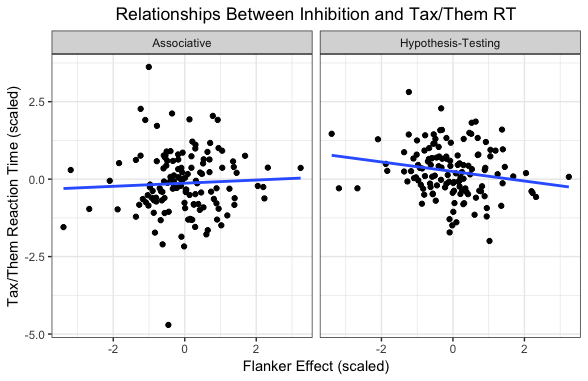
\includegraphics[scale=0.5]{tt_rt_flank.png}
\caption[Relationships between taxonomic/thematic reaction time and vocabulary]{The flanker effect is a significant predictor of reaction time in the taxonomic/thematic task for the hypothesis-testing block, but not for the associative block.}
\label{tt_rt_flank}
\vspace{-10pt}
\end{wrapfigure}		
	
\textbf{Taxonomic/thematic task.}  I constructed a mixed-effects model with random intercepts for subject. Adding the fixed effect of system significantly improved model fit,  $\chi^{2}(1)$ = 18.79, p \textless 0.001. However, adding the individual difference measures did not further improve fit,  $\chi^{2}(4)$ = 0.75, \textit{p} = 0.98. Further, adding the interaction between flanker and system significantly improved fit, $\chi^{2}(1)$ = 5.71, \textit{p} = 0.02. None of the other interactions significantly improved fit. Thus, the final model included random intercepts for subject, main effects for system, RAM, and all the individual difference measures, and an interaction between flanker and system. This model revealed a significant interaction between system and flanker, \textit{F}(1,130) = 5.75, \textit{p} = 0.01 (see Fig \ref{tt_rt_flank}). \par 
	To further break down this model, I ran two follow-up linear models for each of the systems. The model for the hypothesis-testing block showed a significant main effect of flanker, \textit{F}(1,126) = 4.38, \textit{p} = 0.04. The coefficient was negative (\textit{b} = -0.15, \textit{SE} = 0.07), suggesting that individuals with a stronger flanker effect were also slower to respond in the hypothesis-testing block. However, flanker was not a significant predictor in the associative block, \textit{F}(1,126) = 0.30, \textit{p} = 0.59.  \par
\textbf{Summary.} Similar to what was seen in accuracy above, this set of analyses showed that different individual difference measures were related to speed during the three different category learning tasks. Participants with smaller vocabularies responded faster in the associative block of the Ashby task. However, participants with higher accuracy on the Tower of London who responded slower during the associative block of the Sloutsky task. Finally, participants with a smaller flanker effect responded faster on the hypothesis-testing block of the taxonomic-thematic task.

\subsubsection{Exploratory analyses}

While this section is largely devoted to testing the relationship between category learning and individual differences in vocabulary and executive function, two additional individual difference measures were collected (CELF RS and FS). Next I will report the results of analyses investigating the relationship between category learning and these measures. \par
\textbf{Ashby perceptual category learning task.} For both accuracy and reaction time, the base model was a mixed-effects model with random intercepts for subject and fixed effects of system and RAM. Adding the two CELF measures did not significantly improve fit for accuracy, $\chi^{2}(2)$ = 4.24, \textit{p} = 0.12, but they did improve fit for reaction time, $\chi^{2}(2)$ = 7.70, \textit{p} = 0.021. The reaction time model revealed a significant main effect of FS , \textit{F}(1,124) = 7.67, \textit{p} = 0.006 with a positive coefficient (\textit{b} = 0.20, \textit{SE} = 0.07). Thus, participants with better expressive grammar were slower on the Ashby task. \par
\textbf{Sloutsky statistical density task.} For both accuracy and reaction time, the base model was a mixed-effects model with random intercepts for subject and fixed effects of system and RAM. Adding the two CELF measures did not significantly improve fit for accuracy, $\chi^{2}(2)$ = 2.81, \textit{p} = 0.25, or reaction time, $\chi^{2}(2)$ = 0.51, \textit{p} = 0.78. Thus, CELF FS and RS did not predict accuracy or reaction time in this task. \par
\textbf{Taxonomic/thematic task.} The base model for both accuracy and reaction time had random intercepts for subject and fixed effects for system and RAM. CELF FS and RS did not significantly improve model fit for accuracy, $\chi^{2}(2)$ = 0.14, \textit{p} = 0.93, or reaction time, $\chi^{2}(2)$ = 2.15, \textit{p} = 0.34. \par
\textbf{Summary.} These analyses largely show that receptive and expressive grammar were not related to performance in the three category learning tasks in this study. The only significant effect was of FS on reaction time in the Ashby perceptual category learning task. The general lack of results may be influenced by the fact that the participants in this study were at the upper age limit for the CELF (18-21 years) and that they represent a typical (non-language-impaired) population. Thus, this measure may not have been sensitive to fine-grained individual differences in receptive and expressive grammar in this population.

\subsection{Discussion I: individual differences}

	In this section, I tested the core hypothesis of this dissertation, which was that categorization in the hypothesis-testing system relies on executive function while categorization in the associative system relies on verbal labels. I used three category learning tasks and three executive function tasks in addition to measuring vocabulary, which I used as a measure of labeling ability. I expected to find that executive function was strongly related to categorization across tasks in hypothesis-testing blocks but not associative blocks. Conversely, I expected to see strong relationships between associative block performance and vocabulary, but no relationship between hypothesis-testing block performance and vocabulary. \par 
	These hypotheses were not supported by the data. While certain individual difference measures were specifically related to performance in only one system (associative or hypothesis-testing) in each task, the relevant individual difference measures varied by category learning task. In addition, I did not see the hypothesized relationships between vocabulary and the associative system, nor did I see a positive relationship between performance and executive function in most analyses. Since each category learning task differed, I will discuss them separately. \par
	
\subsubsection{Ashby perceptual category learning task}
	In this task, I saw an interaction between vocabulary and performance in both accuracy and reaction time. Participants with larger vocabularies showed higher accuracy in the hypothesis-testing block and slower reaction times in the associative block. While this is the opposite of what I predicted, it is broadly consistent with COVIS if we assume that vocabulary size is broadly related to verbal ability, rather than a specific measure of labeling. Rule-based (hypothesis-testing) categories as described by COVIS must have a verbalizable rule for inclusion; as such, this system is supposed to rely heavily on verbal resources. A study by \citet{Perry2014} found that upregulating activity over Wernicke's area lead to increased use of bi-dimensional categorization strategies. This study used perceptual stimuli (sine wave gratings) that could be categorized either with a uni-dimensional rule, a conjunctive bi-dimensional rule, or an integrative bi-dimensional rule. While the authors report more use of bi-dimensional strategies, they do not indicate which type of bi-dimensional strategy was being used. Given the relationship between language and rule-based category learning in COVIS, this study likely supports the idea that increased recruitment of language resources is related to better bi-dimensional rule-based (rather than integrative) categorization. Thus, the paper by  \citet{Perry2014} is consistent with our results showing that stronger language skills (here, vocabulary) are related to better rule-based categorization ability. \par
	 A similar relationship between language resources and performance was seen for the associative system in this task. Information-integration categories, which are best learned by the associative system, should have no verbal rule for inclusion. Thus, recruiting verbal resources when learning an information-integration category could slow down processing, perhaps by engaging the suboptimal hypothesis-testing system. Indeed, one study showed that when a verbal rule is accessible, the hypothesis-testing system takes over even when it is suboptimal for learning \citep{Noseworthy2011}. Thus, participants with higher vocabularies may recruit verbal hypothesis testing resources in associative blocks which slows down processing. \par
	The lack of significant executive function effects in the Ashby perceptual category task specific to the hypothesis-testing system is not particularly surprising, given the mixed literature on the topic. Some studies do find specific relationships between aspects of executive function and categorization in the hypothesis-testing system in this type of task. \citet{Minda2015} tested some participants on rule-based (hypothesis-testing) and information-integration (associative) categories after they completed a task taxing executive function, while other participants completed an easy task before category learning. They found that the participants with depleted executive function resources showed difficulty learning rule-based categories but not information-integration categories. In addition, \citet{DeCaro2008} found that working memory capacity was positively related to category learning in the hypothesis-testing system but negatively related to category learning in the associative system. However, another study found working memory capacity to be similarly related to both associative and hypothesis-testing category learning \citep{Lewandowsky2012}. Inhibitory control has also been shown to be associated with optimal strategy use for both the associative and hypothesis-testing systems in older adults \citep{Maddox2010}. Thus, the fact that the current study does not find a specific relationship between use of the hypothesis-testing system and executive functioning is in line with the mixed nature of previous literature. However, the fact that no main effects of executive function were found in the Ashby perceptual category learning task is unexpected, as all of the studies cited above did find some relationship between category learning and executive function measures.  \par
	In summary, performance on the Ashby perceptual category learning task was most related to individual differences in vocabulary. Individuals with larger vocabularies showed better performance in the hypothesis-testing system and poorer performance in the associative system. This result is in line with prior research using the COVIS approach, which shows that verbal resources benefit hypothesis-testing but not associative learning of perceptual categories. In addition, this study adds to the mixed literature on the role of executive function in perceptual category learning by providing a null result.
	
\subsubsection{Sloutsky statistical density task}
	The Sloutsky statistical density task showed main effects of inhibition and task-switching on accuracy, and a specific effect of planning on reaction time in the associative block. I will discuss these results; however, caution must be taken in interpreting the accuracy results, as there were considerable ceiling effects in this task. \par
	Better inhibition was related to higher accuracy, while poorer task switching was related to better accuracy. The main effect of inhibition on accuracy is somewhat different from a prior study showing a significant interaction between category sparsity and flanker performance, such that individuals with better inhibition skills also showed faster responses in a picture-word verification task specifically for sparse items \citep{Perry2016}. However, this study used multiple versions of the flanker task where the distractor arrows either appeared simultaneously with the target arrow, 150ms before the target arrow, or 500ms before. This allowed the authors to measure both the cost of incongruent distractors as well as the advantage of congruent distractors. The congruent advantage typically does not appear when the target and distractors are presented simultaneously, as they were in the current study \citep{Botella2002}. It was this congruent advantage, and not the incongruent cost, that the authors found to be specifically related to sparse categorization. Thus, the current study may have been limited by its choice of flanker task; perhaps the interaction between system and inhibition would have been found with a congruent advantage effect rather than the classic flanker effect.  \par 
	The paper by \citet{Perry2016} also looked at how interfering with language resources affected performance on the picture-word verification task. They found that sparse categories were specifically affected by cathodal stimulation over Wernicke's area. That is, interfering with language resources led to slower and less accurate recognition of items from sparse categories, but had no effect on dense categories. Given these results, we might expect that individual differences in vocabulary or language measures like the CELF would be related to performance during hypothesis-testing blocks in the Sloutsky statistical density task. However, none of those effects were found for this task. Instead, the significant predictors were related to executive function. \par 
	All three executive function measures showed some relation to performance in this task. The flanker and switcher effects on accuracy are hard to interpret, given the considerable ceiling effects in this task. However, the specific effect of planning in the associative block is puzzling; it is expected that individuals with better planning skills would be faster at the category learning task, not slower. Additionally, I originally hypothesized that any effects specific to executive function would be found in the hypothesis-testing system, not the associative system. Thus, this interaction was the reverse of my predictions both in direction (better planning = slower) and system (associative rather than hypothesis-testing). In terms of direction, one explanation is that that individuals who exhibited better planning took more time and care in completing assessments, while those with poorer planning completed tasks quickly overall. In the hypothesis-testing block of this task, participants were told which feature to focus on. It is possible that this type of learning does not involve planning; participants could select the feature quickly regardless of their planning ability and overall task speed. In the associative block, there was more of a chance for participants to examine stimuli at different speeds, as no features were highlighted during learning. Thus, the more deliberate participants may have responded slower in this block and performed better during the Tower of London task. Thus, these effects may not reflect strong connections between the constructs of planning and category learning and may instead reflect an overall approach towards the experimental tasks and behavioral measures. \par
	Overall, the results from the Sloutsky statistical density task are hard to interpret. The effects of flanker and switcher on accuracy suffer from ceiling effects, and the effect of planning on reaction time seems to be more related to overall speed of processing than planning specifically. Previously found relationships between individual difference measures and performance on categories of different sparsity were not replicated in this study. This likely stems from significant issues in task and stimulus design that are not addressed in some of the original Sloutsky papers. These issues will be discussed more below.
	
\subsubsection{Taxonomic/thematic task}
	Finally, I saw two effects of executive function on performance in the taxonomic/thematic task. First, there was a main effect of planning on accuracy, such that individuals with higher Tower of London accuracy were also more accurate on the taxonomic/thematic task as a whole. Second, there was a specific effect of inhibition on reaction time in this task. Participants who were better at inhibiting irrelevant information in the flanker task were also faster at responding in the thematic (hypothesis-testing) block. Thus, when there are taxonomic distractors, individual differences in inhibitory control affect reaction time, but this is not the case when the distractors are thematic. This is contrary to findings from an EEG study which found increased power in the upper alpha band \citep{Maguire2010} for taxonomic processing. The authors of this study interpreted these results to indicate increased inhibitory control during taxonomic processing, reflecting effort in inhibiting automatically-activated thematic associates. However, changes in the upper alpha band have also been linked to creativity interventions \citep{Fink2011}, decision-making \citep{Fink2018}, reflection \citep{Rominger2017}, and attention \citep{VanderLubbe2019}. Thus, changes in alpha power during taxonomic but not thematic processing may indicate many processes. As such, the relationship between taxonomic inhibition and inhibitory control found in the current study further contributes to an understanding of the relationship between semantic processing and executive function. \par
	Some previous studies have found other relations between executive function (specifically, cognitive flexibility) and taxonomic/thematic processing. In a few tasks, this was assessed by first reinforcing either taxonomic or thematic relations and then switching to the other type of relation. Studies show that younger school-age children are better at maintaining and switching to a thematic relation than a taxonomic relation, while older adults (ages 60-90) show a specific difficulty in switching to taxonomic relations but no difficulty in maintaining them \citep{Blaye2007, Maintenant2011}. This could suggest that taxonomic relations rely on executive function, such that individuals with poorer executive function (young children and older adults) have more difficulty switching to them. However, these studies do not directly measure individual differences in task switching, so this interpretation is purely speculation. Indeed, it is not borne out by the current results, as no relationships between task switching and performance on the taxonomic/thematic task were found. \par 
	The lack of a relationship between vocabulary or grammar and the taxonomic/thematic task is somewhat unexpected. One study found that production of relational terms at 24 months was related to a thematic preference at 3 years of age \citep{Dunham1995}. Another study found that vocabulary was related to the strength of priming between thematically-related items but not for taxonomically-related items in school-aged children \citep{Brooks2014}. These studies suggest that vocabulary is somewhat related to thematic categorization in childhood. However, it is possible that this relationship disappears by adulthood, when semantic processing and vocabulary skills are more fully developed. This would explain the lack of effects seen in the current study. \par
	The most interesting finding in this analysis was the specific effect of inhibitory control on reaction time in the thematic task. This finding adds to the mixed literature on the effect of executive functions on taxonomic/thematic processing. In addition, no effects were found for vocabulary or grammar, suggesting that these language resources do not modulate performance in taxonomic/thematic processing. Given the relatively abstract nature of this type of semantic processing and the role language plays in thought, this finding is surprising. 
	
\subsubsection{Limitations and conclusions}	

	While this study was designed with many considerations in mind, it is certainly not without its flaws. One limitation of this study was the choice to use vocabulary as a measure of labeling. I chose this measure instead of a paired-associate learning task because I was interested in elaborated links between meanings and labels rather than just memory for labels. However, adding a paired-associate learning task in addition to the vocabulary measure could have provided a deeper understanding of the relationship between labeling and category learning in the two systems. Additionally, the grammar measure (CELF) showed limited variability in this sample. Grammar and syntax are certainly important for word form and meaning learning during development, so it is possible that the limited variability contributed to the mostly null findings regarding this measure and category learning. A measure of working memory capacity would also have served to broaden the study's examination of category learning and executive function. Finally, as described in Experiment 1, the Sloutsky statistical density task would have benefited from careful examination and norming of stimuli. \par
	Another more general limitation of this study is its use of cognitive experimental tasks to conduct an individual differences analysis. This issue is described and tested in \citet{Hedge2018}. The general idea is that many experimental tasks are designed to minimize individual differences to produce a robust group or condition effect. Reliable tasks that are sensitive to individual differences are often discarded, as the experimental effect of interest is obscured by the individual differences and thus considered not robust. The paper cited above found low intraclass correlations between different testing instances in the same subjects for many commonly used experimental tasks. For example, they found ICCs as low as 0.40 for the flanker task, a task used in the current study. Since many of the findings from the current study are relatively novel and conducted on a single sample, replication is needed before strong conclusions can be made. Finally, multivariate approaches that can include all the individual difference measures as well as all the category learning tasks in a single model would provide additional insight into the relationships among these measures. \par
	Despite these limitations, this study takes a step towards understanding individual differences in category learning. A striking pattern revealed in this analysis is that different individual difference measures were related to performance on the three category learning tasks. Even those measures that showed relationships to more than one category learning task (e.g., planning) had different relationships with each task. Thus, not only was the core hypothesis not supported from this investigation, but the comparability of these three paradigms for studying category learning is not apparent. In other words, this analysis suggests that different skills underlie each of the three category learning tasks. To further address this issue, the next analysis will directly compare performance on the three category learning tasks without taking into account individual difference measures.
	 
	
\subsection{Results II: cross-paradigm comparison}

For descriptive statistics on subject- and block-wise aggregated accuracy and reaction time in the category learning tasks, see Tables \ref{cross_comp_acc_desc} and \ref{cross_comp_rt_desc}.
\begin{table}[H]
\caption{Descriptive statistics for category learning tasks (subsample) -- accuracy.}
\vspace{-10pt}
\begin{center}
\begin{tabularx}{\textwidth}{>{\centering\arraybackslash}p{4.5cm}YYYYYY}
\toprule
\multirow{2}{*}{Paradigm}    & \multicolumn{3}{c}{Associative} & \multicolumn{3}{c}{Hypothesis-testing} \\
                             & Mean    & SD      & Range       & Mean      & SD        & Range          \\
\midrule
Ashby perceptual             & 0.58    & 0.07    & 0.46-0.76   & 0.81      & 0.14      & 0.45-0.97      \\
Sloutsky statistical density & 0.95    & 0.09    & 0.6-1.00    & 0.92      & 0.15      & 0.2-1.0        \\
Taxonomic/thematic           & 0.84    & 0.13    & 0.21-1.00   & 0.84      & 0.16      & 0.21-1.00     \\
\bottomrule 
\label{cross_comp_acc_desc}
\end{tabularx}
\end{center}
\vspace{-10pt}
\small\textit{Note}. Only the 84 subjects included in the cross-paradigm analyses are summarized in this table.
\end{table}


\begin{table}[H]
\caption{Descriptive statistics for category learning tasks (subsample) -- reaction time.}
\vspace{-10pt}
\begin{center}
\begin{tabularx}{\textwidth}{>{\centering\arraybackslash}p{4.5cm}YYYYYY}
\toprule
\multirow{2}{*}{Paradigm}    & \multicolumn{3}{c}{Associative} & \multicolumn{3}{c}{Hypothesis-testing} \\
                             & Mean    & SD      & Range       & Mean      & SD        & Range          \\
\midrule
Ashby perceptual             & 738    & 250    & 122-1780 & 621      & 134      & 131-1030      \\
Sloutsky statistical density & 792    & 206    & 431-1320 & 667      & 151      & 413-1210        \\
Taxonomic/thematic           & 1730    & 752    & 786-6030 & 1920      & 545      & 918-3500     \\
\bottomrule 
\label{cross_comp_rt_desc}
\end{tabularx}
\end{center}
\vspace{-10pt}
\small\textit{Note}. Only the 84 subjects included in the cross-paradigm analyses are summarized in this table.
\end{table}

\subsubsection{Data processing}

Concordant with an \textit{a priori} power analysis and pre-registration, only the first 84 undergraduate students with complete data were included in the analyses reported in this section. Recall that the relationships between task conditions and the two categorization systems are summarized in Table \ref{exp2systems}. \par
	\textbf{Ashby perceptual category learning task.} Accuracy and reaction time were measured for this task. Accuracy was summarized by subject and system. For reaction time, only accurate trials were used. Outliers were removed on a by-trial basis using the same method described in the individual differences analysis. Then, reaction time was summarized by subject and system. Next, I constructed boxplots to summarize mean RTs for each system and paradigm. Subjects who were clear outliers for both systems within a given paradigm were excluded (1 participant) and replaced with the next participant. Accuracy and reaction time were then Yeo-Johnson transformed to reduce skewness, as well as centered and scaled. At this point, any subjects with a z-score of less than -3 or greater than 3 were considered outliers and removed from further analysis. \par
	\textbf{Sloutsky statistical density task.} Any participants who did not respond correctly to at least 6 of the 8 catch trials for a given block were removed from future analyses. Thus, all subjects reported in analyses using this task had at least 75\% accuracy on catch trials in both blocks. Accuracy was summarized by subject and system. Reaction time outliers were removed on a by-trial basis as described above and reaction time was then summarized by subject and system. Next, I constructed boxplots to summarize mean RTs for each system and paradigm. No subjects for this task were clear outliers. Accuracy and reaction time were then transformed, centered, and scaled. At this point, any subjects with a z-score of less than -3 or greater than 3 were considered outliers and removed from further analysis. \par
	\textbf{Taxonomic/thematic task.} Practice trials were discarded before analysis. Accuracy was summarized by subject and system. Reaction time outliers were removed using the same method as above, and then reaction time was summarized by subject and system. Next, I constructed boxplots to summarize mean RTs for each system and paradigm. Subjects who were clear outliers for both systems within a given paradigm were excluded (2 participants) and replaced with the next 2 participants. Accuracy and reaction time were then transformed, centered, and scaled. At this point, any subjects with a z-score of less than -3 or greater than 3 were considered outliers and removed from further analysis. \par	
	
\begin{table}[H]
\caption{Correlations between category learning tasks -- accuracy.}
\vspace{-10pt}
\begin{center}
\begin{tabularx}{\textwidth}{p{6cm}YYYYYY}
\toprule
\multicolumn{1}{c}{Task}           & 1     & 2    & 3     & 4     & 5    & 6 \\
\midrule
1. HT Ashby perceptual             & -     &      &       &       &      &   \\
2. HT Sloutsky statistical density & 0.21  & -    &       &       &      &   \\
3. HT Taxonomic/thematic           & -0.07 & 0.18 & -     &       &      &   \\
4. AS Ashby perceptual             & 0.37* & 0.12 & 0.00  & -     &      &   \\
5. AS Sloutsky statistical density & 0.19  & 0.08 & 0.06  & 0.14  & -    &   \\
6. AS Taxonomic/thematic           & 0.05  & 0.14 & 0.39* & -0.12 & 0.23 & - \\
\bottomrule
\label{catlearn_corr_acc}
\end{tabularx}
\end{center}
\vspace{-10pt}
\small\textit{Note}. Only the 84 subjects included in the cross-paradigm analyses are included in this table. HT = hypothesis-testing, AS = associative. * \textit{p} \textless 0.05, Bonferroni corrected.
\end{table}		

\begin{table}[H]
\caption{Correlations between category learning tasks -- reaction time.}
\vspace{-10pt}
\begin{center}
\begin{tabularx}{\textwidth}{p{6cm}YYYYYY}
\toprule
\multicolumn{1}{c}{Task}           & 1     & 2    & 3     & 4     & 5    & 6 \\
\midrule
1. HT Ashby perceptual             & -     &       &       &       &      &   \\
2. HT Sloutsky statistical density & 0.30  & -     &       &       &      &   \\
3. HT Taxonomic/thematic           & 0.24  & 0.36* & -     &       &      &   \\
4. AS Ashby perceptual             & 0.58* & 0.25  & 0.24  & -     &      &   \\
5. AS Sloutsky statistical density & 0.29  & 0.49* & 0.26  & 0.31  & -    &   \\
6. AS Taxonomic/thematic           & 0.13  & 0.22  & 0.54* & 0.19  & 0.23 & - \\
\bottomrule
\label{catlearn_corr_rt}
\end{tabularx}
\end{center}
\vspace{-10pt}
\small\textit{Note}. Only the 84 subjects included in the cross-paradigm analyses are included in this table. HT = hypothesis-testing, AS = associative. * \textit{p} \textless 0.05, Bonferroni corrected.
\end{table}	
	
\subsubsection{Accuracy}
To investigate whether accuracy was comparable across paradigms, I constructed a mixed-effects model with random intercepts for subject. Adding the fixed effects of paradigm and system significantly improved model fit, $\chi^{2}(3)$ = 32.24, \textit{p} \textless 0.0001. Adding the interaction between paradigm and system further increased fit, $\chi^{2}(2)$ = 75.60, \textit{p} \textless 0.0001. Thus, the final model predicted the accuracy z-scores from paradigm, system, and their interaction. This model revealed a significant main effect of system, \textit{F}(1,415) = 38.37, \textit{p} \textless 0.0001, as well as a significant interaction between paradigm and system, \textit{F}(2,415) = 41.00, \textit{p} \textless 0.0001 (see Fig \ref{h2_acc}). To further investigate this interaction, I conducted three follow-up models, each testing the effect of system within a given paradigm. \par
	The first model revealed a significant main effect of system in the perceptual category learning paradigm, \textit{F}(1,83) = 210.27, \textit{p} \textless 0.0001. A follow-up t-test confirmed that accuracy was significantly higher for the hypothesis-testing system, \textit{t}(133) = -11.90, \textit{p} \textless 0.0001. The second model revealed no main effect of system in the statistical density paradigm, \textit{F}(1,83) = 0.92, \textit{p}  = 0.34. A follow-up t-test confirmed this result, \textit{t}(135) = 0.91, \textit{p}  = 0.36.  Finally, the third model showed no main effect of system in the taxonomic-thematic paradigm, \textit{F}(1,83) = 0.73, \textit{p}  = 0.40. This was confirmed by a follow-up t-test, \textit{t}(164) = -0.66, \textit{p}  = 0.51. \par
	
\begin{figure}[h]
\begin{center}
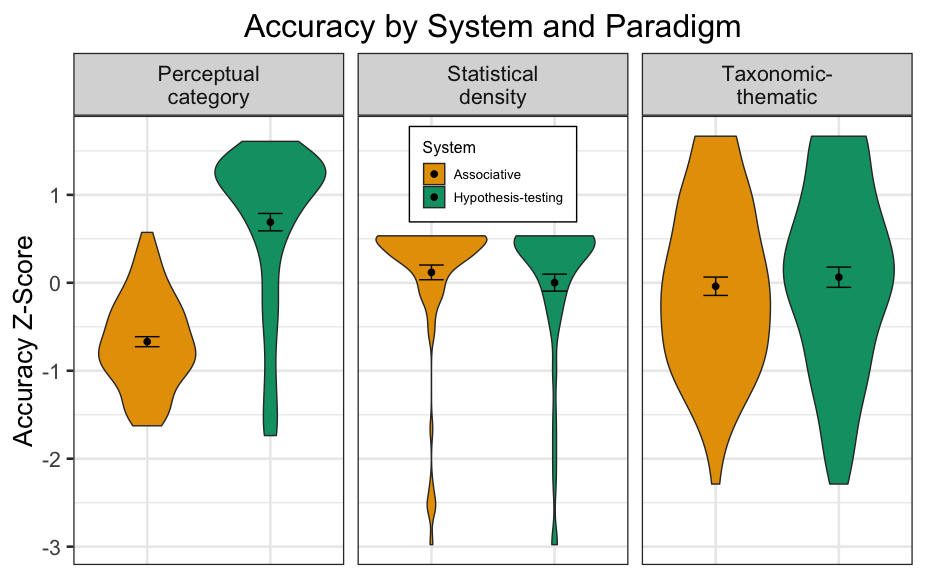
\includegraphics[scale=0.45]{h2_acc}
\caption[Accuracy results for cross-paradigm comparison]{Accuracy results for cross-paradigm comparison analysis. Points indicate means with error bars reflecting standard error. Shaded portions represent the distribution of accuracy \textit{z}-scores.}
\vspace{-20pt}
\label{h2_acc}
\end{center}
\end{figure}	
	
	Overall these results suggest that these three paradigms are not comparable. While no differences between systems were found for the statistical density and taxonomic-thematic tasks, the perceptual category learning task showed a different pattern. However, the statistical density task may have been suffering from ceiling effects. Of the 84 total subjects, average accuracy values were 0.9 or higher during the statistical density paradigm in 76 subjects for the associative block and 58 subjects for the hypothesis-testing block. Thus, the statistical density task may not be sufficiently difficult to detect differences between systems in accuracy.
 \par
\subsubsection{Reaction time}
To investigate whether reaction time was comparable across paradigms, I constructed a mixed-effects model with random intercepts for subject. Adding the fixed effects of paradigm and system significantly improved model fit,  $\chi^{2}(3)$ = 13.48, p = 0.003. Adding the interaction between paradigm and system further increased fit,  $\chi^{2}(2)$  = 44.65, \textit{p} \textless 0.0001. Thus, the final model predicted the accuracy z-scores from paradigm, system as well as their interaction. This model revealed a significant main effect of system, \textit{F}(1,415) = 14.62, \textit{p} = 0.0001, but no main effect of paradigm, \textit{F}(2,415) = 0.017, \textit{p} = 0.84. The interaction between system and paradigm was also significant, \textit{F}(2,415) = 23.30, \textit{p} \textless 0.0001 (see Fig \ref{h2_rt}). To further investigate this interaction, I conducted three follow-up models each testing the effect of system within a given paradigm. \par
	The first model revealed a significant main effect of system in the perceptual category learning paradigm, \textit{F}(1,83) = 29.96, \textit{p} \textless 0.0001. A follow-up t-test confirmed that reaction time was significantly faster for the hypothesis-testing system, \textit{t}(141) = 3.73, \textit{p} = 0.0002. The second model revealed a significant main effect of system in the statistical density paradigm, \textit{F}(1,83) = 44.00, \textit{p} \textless 0.0001. A follow-up t-test showed that again reaction time was faster for the hypothesis-testing system, \textit{t}(165) = 4.62, \textit{p} \textless 0.0001.  Finally, the third model also showed a main effect of system in the taxonomic-thematic paradigm, \textit{F}(1,83) = 14.96, \textit{p} = 0.0002. However, for this paradigm the pattern was flipped. Reaction times were faster for the associative system, \textit{t}(162) = -2.68, \textit{p} = 0.008.
	
\begin{figure}[h]
\begin{center}
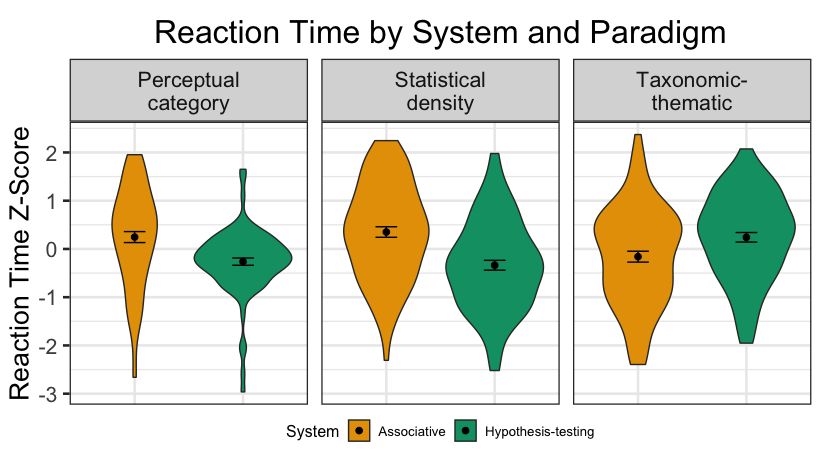
\includegraphics[scale=0.55]{h2_rt}
\caption[Reaction time results for cross-paradigm comparison]{Reaction time results for cross-paradigm comparison analysis. Points indicate means with error bars reflecting standard error. Shaded portions represent the distribution of reaction time \textit{z}-scores.}
\vspace{-20pt}
\label{h2_rt}
\end{center}
\end{figure}		
	
	
\subsection{Discussion II: Cross-paradigm comparison}

This analysis aimed to directly compare three dual-systems approaches to category learning. From a theoretical standpoint, considerable similarities can be drawn between these approaches. They each consider two category structure types, which can be mapped onto similarity- and rule-based categories. In addition, two of the approaches posit very similar systems for learning these categories, each specifically adapted to a single category type. The associative system best learns similarity-based categories by integrating and compressing multiple features using an iterative and associative process. The hypothesis-testing system uses higher-order skills like working memory and executive functions to select and test hypotheses about category-relevant features. This system is best for learning rule-based categories. Each approach uses a different paradigm to measure how individuals learn these different category structures. I hypothesized that while there are considerable task-related differences among the paradigms from each approach, each paradigm would engage the relevant category learning system in a given block. Thus, I expected to see a main effect of system but no effect of paradigm, indicating that each task separately engaged the two systems in different blocks. \par
	I did not find these hypothesized results in either accuracy or reaction time. In accuracy, two of the paradigms showed no differences between systems while one showed a different pattern. For the Ashby perceptual category learning task, accuracy was much lower for the associative system than for the hypothesis-testing system. In fact, mean accuracy in the associative block of this task was barely above chance, indicating that participants may not have even learned these categories. In contrast, no accuracy differences were seen between the two blocks in the taxonomic/thematic and Sloutsky statistical density task. The Sloutsky statistical density paradigm also suffered from considerable ceiling effects. In reaction time, I again saw paradigm-related differences. In both the Ashby perceptual category learning task and the Sloutsky statistical density task, participants were significantly faster in the hypothesis-testing block than in the associative block. However, this pattern was reversed for the taxonomic/thematic task. In the next section, I will discuss some of the task-specific factors that may have contributed to the differences in performance seen across the three tasks. \par
	
\subsubsection{Task differences}

\textbf{Stimuli.} One of the most striking differences between Ashby, Sloutsky, and taxonomic/thematic tasks is the stimuli. Almost all papers following the COVIS model use sine-wave grating/Gabor patch stimuli, where the only varying features are orientation and frequency. This type of stimulus is largely meaningless, although some papers attempt to map it onto more meaningful categories like alien eyes, minerals, or flowers \citep{Tolins2015, Perry2014}. However, in most studies it is difficult to connect a sine-wave grating stimulus to existing category knowledge. Previous research has shown that even minimal prior knowledge can facilitate category learning, \citep{Kaplan2000}. In addition, providing information about individual features (even without explicitly linking them to categories) helps participants attend to category-relevant features in subsequent category learning \citep{Kim2011}. Thus, meaningless categories like the sine-wave gratings should be harder to learn than the novel stimuli in the Sloutsky statistical density task, which were based on existing categories (e.g., flowers). \par
	This assumption is supported both by prior research and the current results. In one COVIS-based study, participants only achieved a mean accuracy of 79\% for information-integration (associative) stimuli, 93\% for simple rule-based (hypothesis-testing) stimuli, and 82.1\% for complex rule-based (hypothesis-testing) stimuli \citep{Helie2010}. In contrast, similarity-based stimuli from \citet{Kloos2008} were learned with almost perfect accuracy after viewing just 16 instances, and rule-based stimuli were learned to about 75\% accuracy (taking into account false alarm responses) after a single encounter with the category rules. In the current study, accuracy was lower in the Ashby perceptual category learning task than in the other two tasks overall. This perhaps suggests that perceptual categories are learned in a different manner or on a different time scale than categories that are connected to meaning, like those used in the Sloutsky statistical density and taxonomic/thematic tasks. \par
	An interesting thing to note is that dense (associative) stimuli used in the Sloutsky statistical density task would be considered rule-based under COVIS. Recall that the two core features of rule-based stimuli under COVIS are that the rules for inclusion are easily verbalizable and that the learner can make a decision on each feature separately before their combination. This is certainly the case for the dense (associative) statistical density stimuli used in the current study (e.g., aliens with small bodies and big feet and curly hair and few teeth, etc.). None of the dimensions need to be integrated before making a category decision; the conjunctions linking them (“and”) do that work instead. Thus, from a COVIS perspective, all of the stimuli used in the current Sloutsky statistical density task are rule-based, albeit with varying numbers of relevant dimensions. This may explain the large discrepancy between accuracy in the associative blocks for the Ashby and Sloutsky tasks – the former was close to chance while the latter was nearer to ceiling. Rule-based (hypothesis-testing) stimuli from the COVIS approach are consistently easier to learn; participants show higher accuracy for these stimuli than for information-integration (associative) stimuli in most if not all studies. Thus, perhaps all of the stimuli in the current Sloutsky statistical density are in fact tapping the hypothesis-testing system, leading to no differences in accuracy between the two blocks. \par
	Finally, the stimuli used in the taxonomic/thematic task are in some ways fundamentally different than those used in the other tasks. Participants in this study took more than twice as long on average to respond to taxonomic/thematic stimuli than to Ashby perceptual or Sloutsky statistical density stimuli. They also are the only stimuli that include real-world objects; the other tasks used stimuli constructed specifically for the experiment. Another core difference is that taxonomic and thematic categories can be somewhat overlapping. For example, horses and sheep are both animals (taxonomic) but they also are commonly found together in a farming scenario (thematic). Thus, it is possible that individuals use both the hypothesis-testing and the associative systems to process taxonomic and thematic categories. This is in direct contrast to perceptual categories, which by design can only be learned with a certain type of strategy, and statistical density categories, which have a clear ideal system depending on their density. \par
\textbf{Task Demands.} In creating this study, I chose to use common paradigms from each approach. I selected this strategy because I wanted to see if each approach as it currently stands was engaging the two category learning systems in the same way. However, this lead to some core differences in task structure, the most important of which being the learning procedure. In the Ashby perceptual learning task, participants had no training period. They were told from the beginning that they would be learning novel categories, initially starting with trial and error. Each trial of this task was a test trial, and each trial included feedback. In contrast, each block of the Sloutsky statistical density task had a training period where category information was presented to the participant, and a testing period where no feedback was present. The taxonomic/thematic task was somewhere in between. It had both training and testing with feedback present for both. Thus, learning demands differed for all three tasks. \par 
Prior research has compared different types of learning tasks for perceptual categories \citep{Ashby2002}. In this study, some participants learned hypothesis-testing and associative categories in the same feedback-based paradigm used in the current study. Other participants saw exemplars from a given category and were told which category these exemplars belonged to, similar to the way participants learned associative categories in our Sloutsky statistical density task. They found that participants could learn hypothesis-testing categories in both learning conditions. However, participants showed difficulty learning the associative categories in the exemplar-based training. Another study found feedback learning to be superior to exemplar-based learning for both types of categories \citep{Edmunds2015}. In our study, participants were nearly at ceiling for learning associative categories using exemplar-based training in the Sloutsky statistical density task. This suggests that even if learning demands were equated across tasks, performance would still not be equivalent for the different types of stimuli.
	
\subsubsection{Limitations and conclusions}

	As discussed above, one of the limitations to this study is that it used different types of tasks in each paradigm. That makes it hard to disentangle whether the paradigm-related differences seen in this study are due to dissimilarities between the theories each paradigm is trying to test or simple task differences. Future studies would benefit from greater control of task demands. Additionally, the concerns about stimulus norming discussed in Experiment 1 also apply to this experiment, as the stimuli used in the Sloutsky statistical density task for both experiments were the same. More careful examination of feature salience and relations among features would make it easier to compare these stimuli to sine-wave gratings and taxonomic/thematic categories. \par
	A key takeaway from this study is that despite the theoretical similarities behind these approaches, the tasks they use to measure category learning are not directly comparable. Even after accounting for scaling considerations by using \textit{z}-scores, the relationship between category learning in the two systems is not consistent across paradigms. As discussed above, this could simply be explained by task and stimuli differences; perhaps each approach is indeed trying to measure the same types of processing, but they are taxing the systems differently. Another possibility is that each approach is fundamentally trying to explain different, albeit related, phenomena. I will consider the second possibility in the general discussion.

\end{document}

